\chapter{Supplementary materials for:\\Spatially shifting temporal points: estimating pooled within-time series variograms for scarce hydrological data}
\label{appendixB}

\section{Supplementary computer code and data}
\label{Supplementary computer code and data}

The computer code along with the reference manual for estimating pooled within-time series (PTS) variograms by applying newly developed spatially shifting temporal points (SSTP), available  averaging empirical variograms (AEV) and a modification of AEV, i.e. weighted averaging empirical variograms (WAEV) methods, is available with the digital version of this thesis and from an online repository: \href{https://github.com/AvitBhowmik/SSTP}{https://github.com/AvitBhowmik/SSTP}. The computer code is an R-script that uses the provided sample data (with the digital version of thesis and the above repository) as input and provides the estimation of PTS variograms by above methods as output. The script was tested using the latest R version 3.2.0 -- ``Full of Ingredients'' that was released on 16.04.2015. Installation of three packages are required: ``spacetime'', ``intamap'' and ``gstat'', where installation of ``intamap'' requires pre-installation of the dependency packages: ``mvtnorm'', ``evd'' and ``sp''. The dependencies may also be automatically installed by R while installing the packages. The installation guideline is provided in the script. Further details and documentations on R and the packages are available from: \href{http://www.r-project.org/}{http://www.r-project.org/}. To get familiar with R, usage examples are available from: \href{http://tryr.codeschool.com/levels/1/challenges/1}{http://tryr.codeschool.com/levels/1/challenges/1}.

The sample data contains computed annual total precipitation in hydrological wet days (PRCPTOT) values at the available data points in Bangladesh for 1993-2007 series. This is a ``STFDF'' data and provided in ``.Rdata'' format. Details on the data format, instructions on how to read and analyze the data are provided in the R-script and package vignettes.

\section{Supplementary figure and table}
\label{Supplementary figure and table}

Figure B.1 illustrates the change in spatial location, distribution and density of the available data points for PRCPTOT in Bangladesh within the 1948-2007 series. A sample of four representative years, i.e. 1948, 1966, 1983 and 2007, is also integrated in Figure 3.3 in chapter 3.

Table B.1 presents the change in the number of available data points and data density, smallest and largets spatial-lags and summary statistics, i.e. minimum, mean, maximum and coefficient of variation of annual total precipitation in hydrological wet days (PRCPTOT) in Bangladesh within the 1948-2007 series. A sample of four representative years, i.e. 1948, 1966, 1983 and 2007, is presented in Figure 3.3 in chapter 3.

\begin{figure*}[h!]
  \centering
  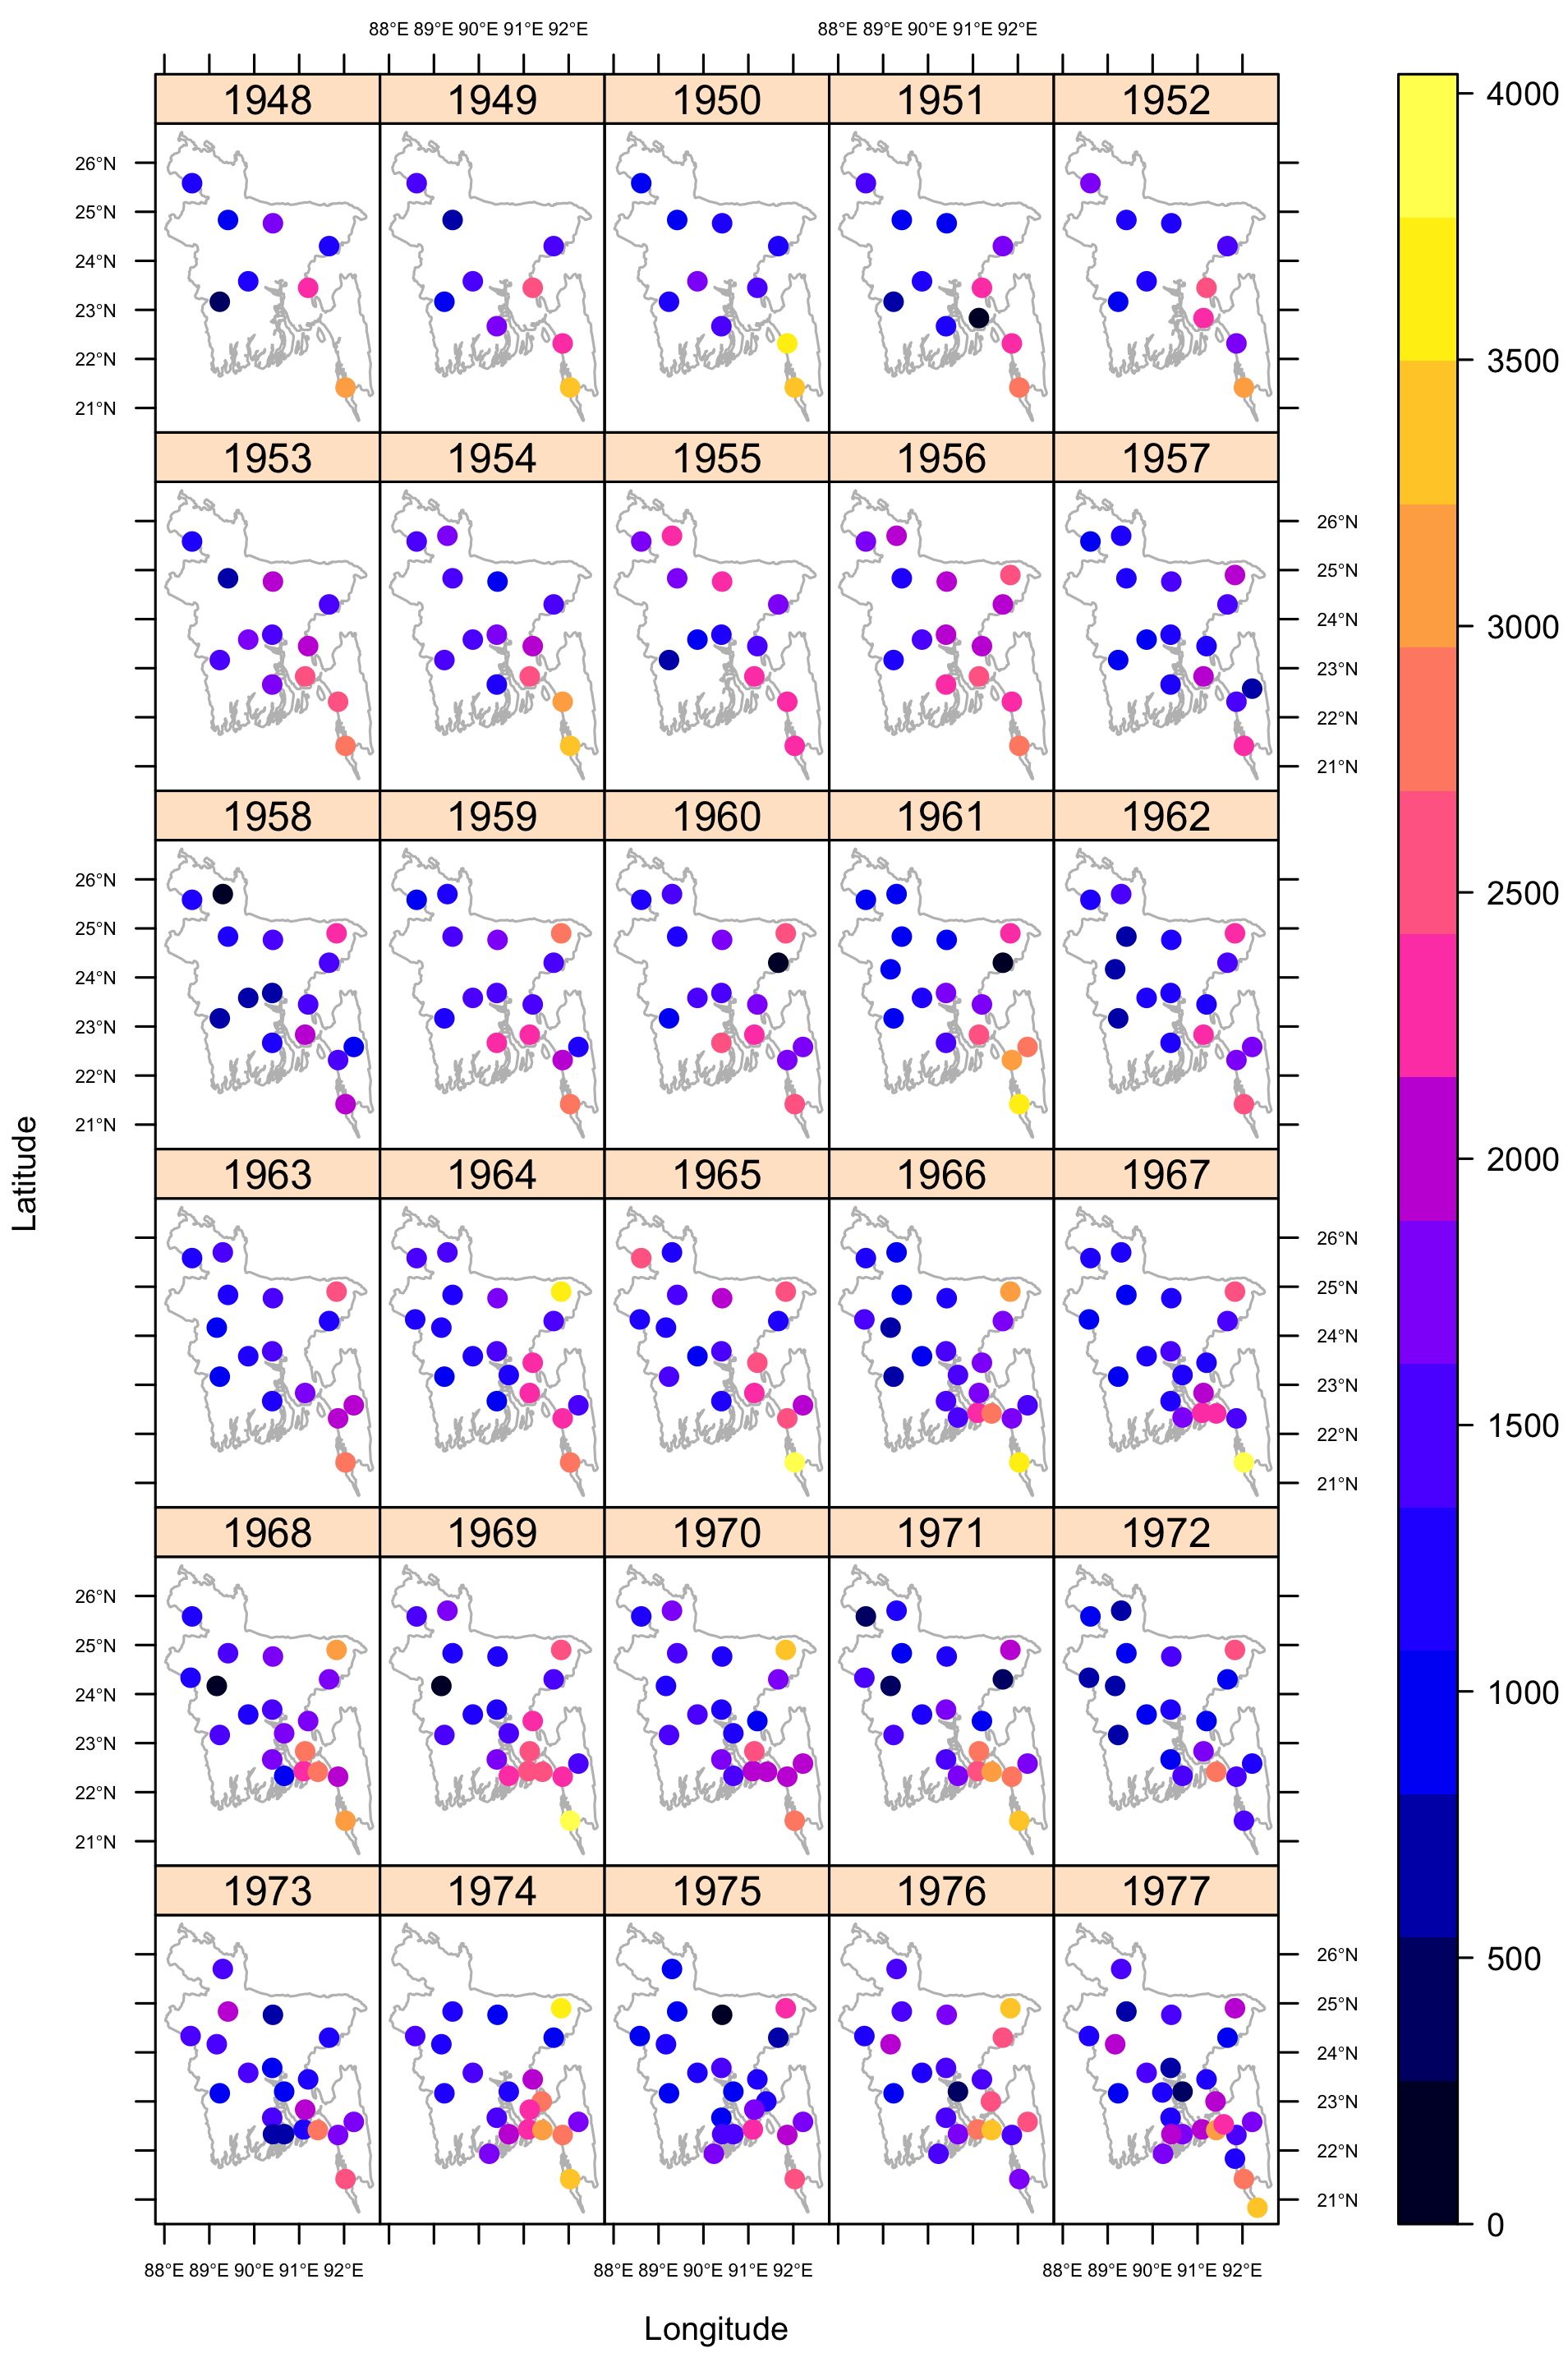
\includegraphics[width=\textwidth]{Figures/Fig_B_1_a.png}
  \label{Fig_B_1_a}
\end{figure*}

\begin{figure}[h!]
  \centering
  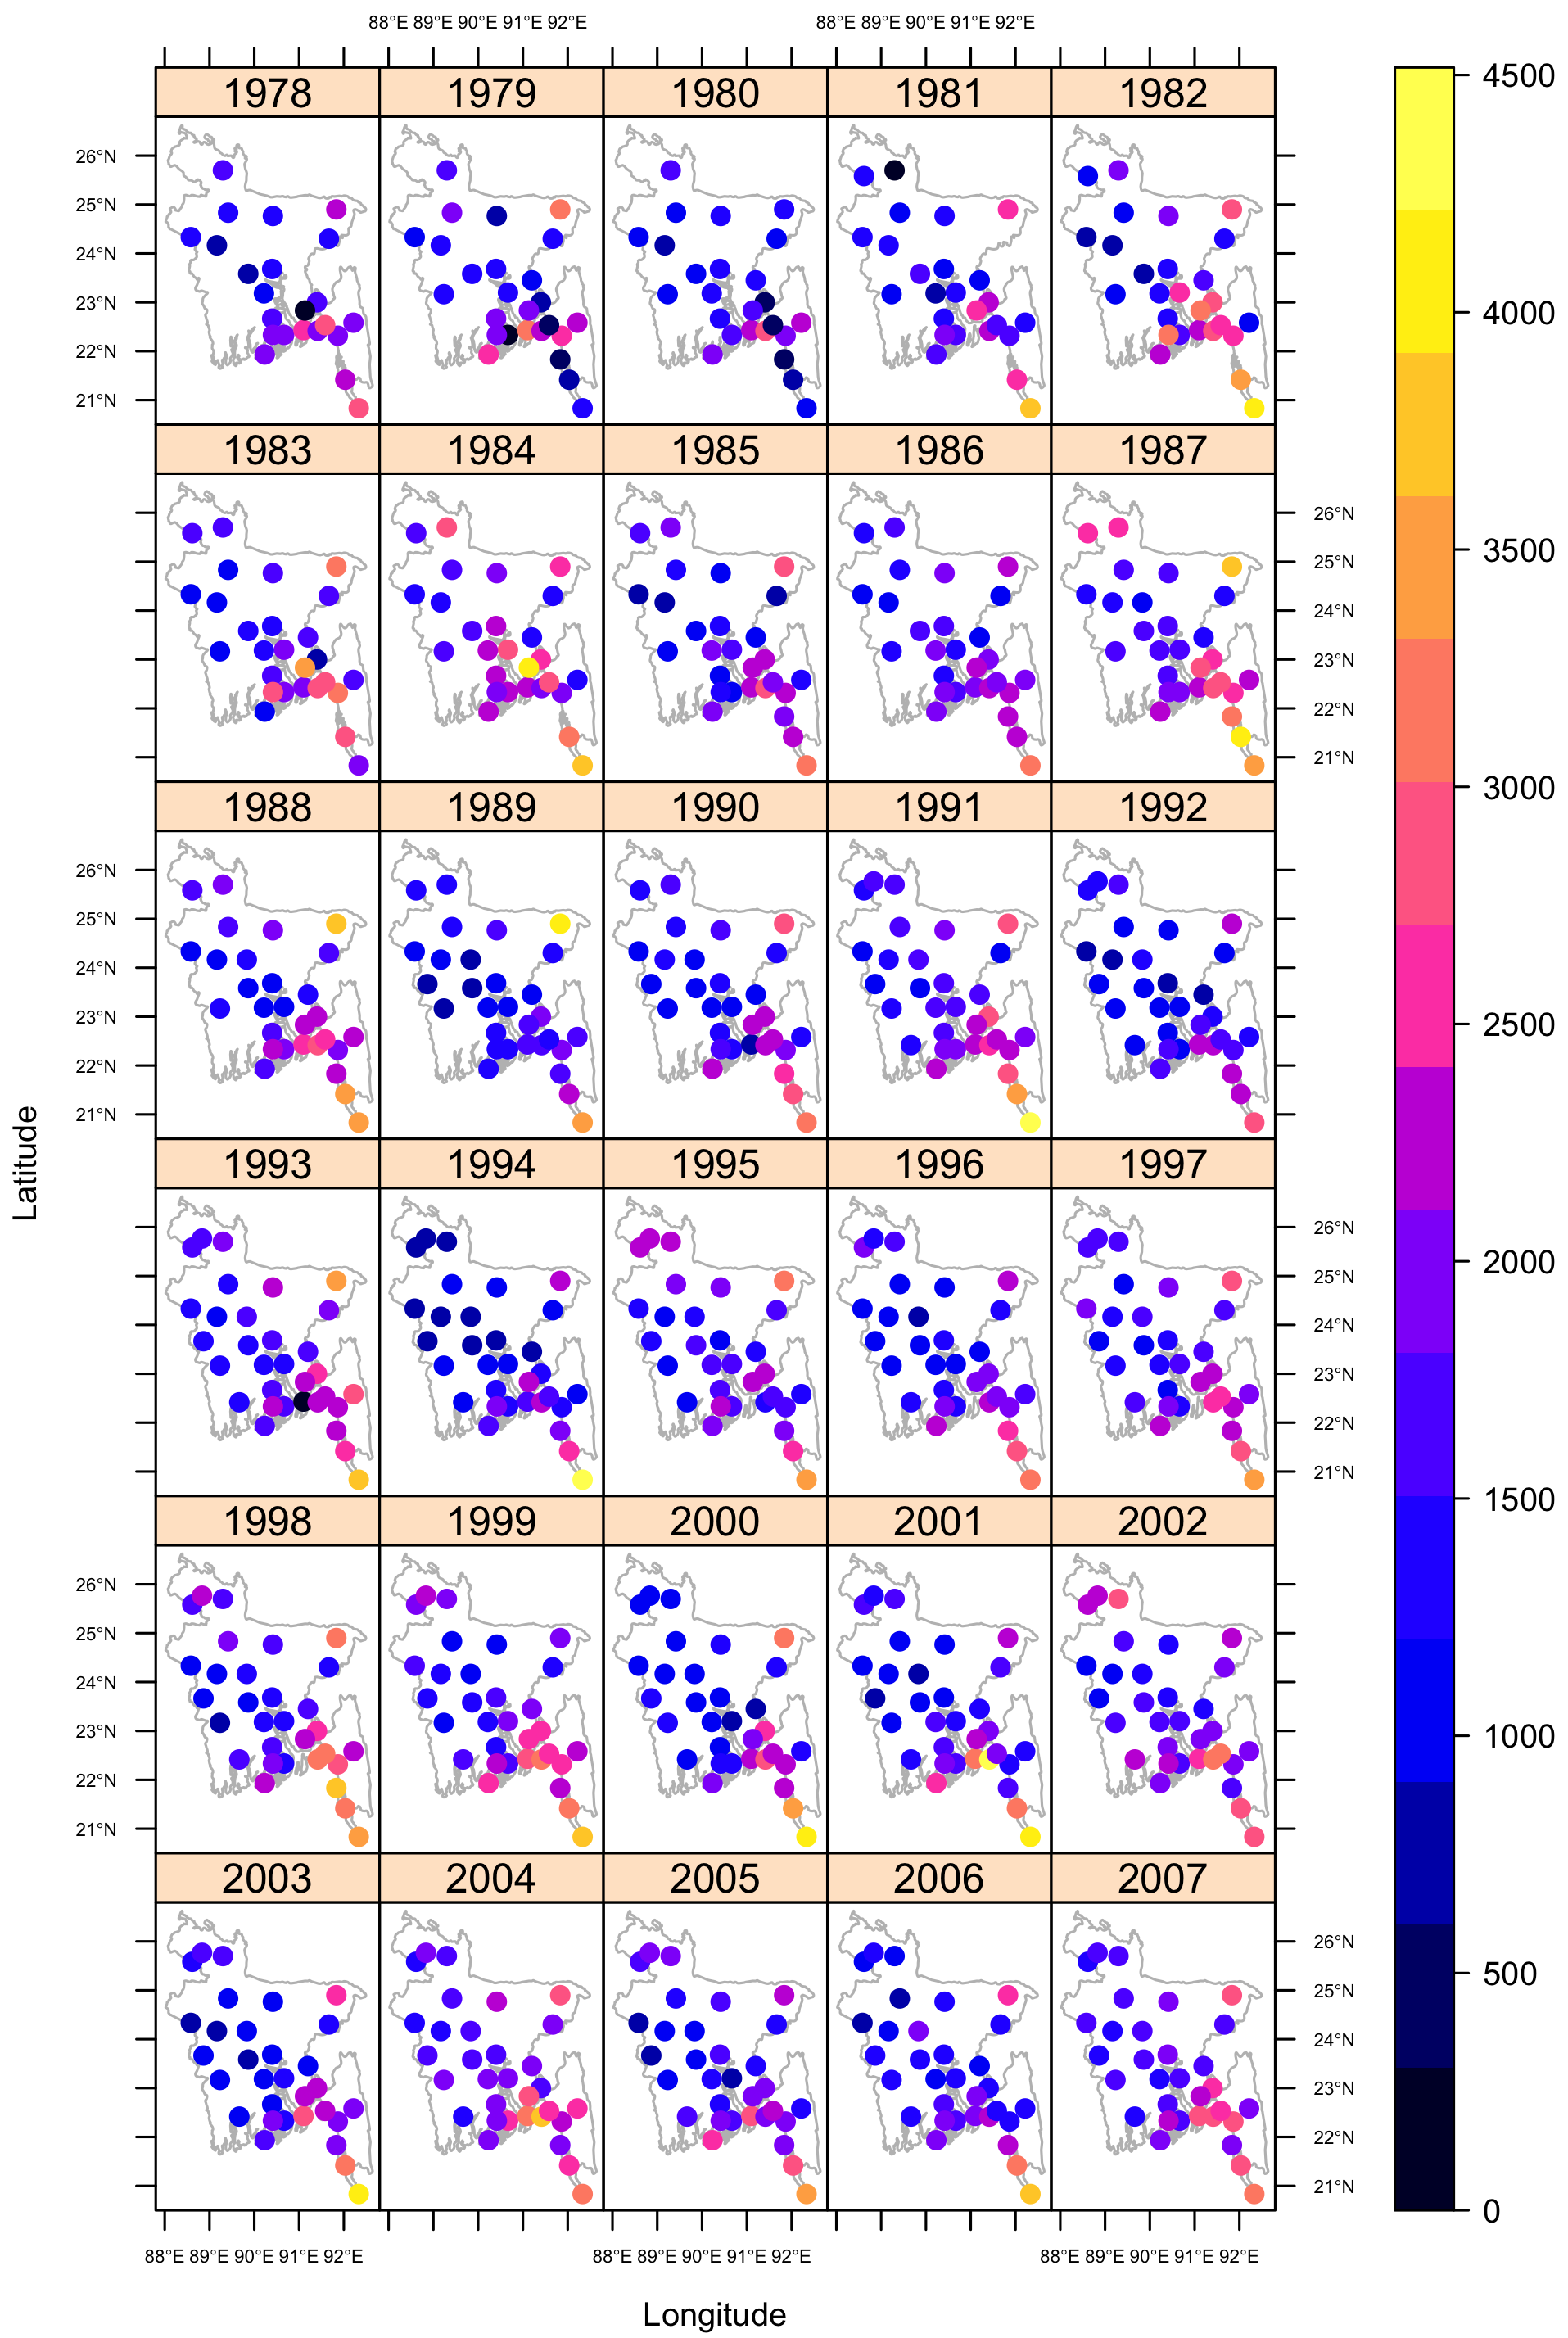
\includegraphics[width=\textwidth]{Figures/Fig_B_1_b.png}
  \caption{Spatial location, distribution and density of available data points (rain-gauge) for each year and annual total precipitation in hydrological wet days (PRCPTOT) (in mm).}
  \label{Fig_B_1_b}
\end{figure}

\clearpage

\setlength{\LTcapwidth}{\linewidth}

\begin{longtable}[c]{>{\centering\arraybackslash}m{0.7cm}>{\centering\arraybackslash}m{2.0cm}>{\centering\arraybackslash}m{2.5cm}>{\centering\arraybackslash}m{1.0cm}>{\centering\arraybackslash}m{1.0cm}>{\centering\arraybackslash}m{0.7cm}>{\centering\arraybackslash}m{0.7cm}>{\centering\arraybackslash}m{0.7cm}>{\centering\arraybackslash}m{0.7cm}}

\caption{Number of available data points, data point density, smallest and largest spatial-lags, and minimum (min.), mean, maximum (max.) and coefficient of variation (CV) of annual total precipitation in hydrological wet days (PRCPTOT) in Bangladesh for each time step (year) within 1948-2007 series.}

\hline
\textbf{Year} & \textbf{Available number of data points} & \textbf{Data point density} & \multicolumn{2}{c}{\textbf{Spatial lag}} & \multicolumn{4}{c}{\textbf{PRCPTOT}}\\
 & & & \textbf{Smallest} & \textbf{Largest} & \textbf{Min.} & \textbf{Mean} & \textbf{Max.} & \textbf{CV}\\
 & & \textbf{(point/10000 $km^2$)} & \textbf{$(km)$} & \textbf{$(km)$} & \textbf{$(mm)$} & \textbf{$(mm)$} & \textbf{$(mm)$} & \textbf{(\%)}\\
\hline
\endfirsthead

\hline
\endhead

\hline
\endfoot

1948 & 8 & 0.5 & 95.38 & 489.85 & 494 & 1532 & 3028 & 53.59\\
1949 & 9 & 0.6 & 95.22 & 489.85 & 574 & 1772 & 3369 & 47.40\\
1950 & 10 & 0.7 & 96.76 & 489.85 & 981 & 1708 & 3521 & 54.98\\
1951 & 11 & 0.7 & 68.57 & 489.85 & 225 & 1447 & 2916 & 53.77\\
1952 & 10 & 0.7 & 68.57 & 489.85 & 972 & 1778 & 3131 & 37.96\\
1953 & 12 & 0.8 & 62.08 & 489.85 & 671 & 1818 & 2813 & 32.95\\
1954 & 13 & 0.9 & 64.69 & 549.70 & 1006 & 1876 & 3378 & 36.73\\
1955 & 12 & 0.8 & 64.69 & 549.70 & 779 & 1744 & 2374 & 31.25\\
1956 & 14 & 0.9 & 65.64 & 549.70 & 1214 & 2016 & 2913 & 24.55\\
1957 & 15 & 1.0 & 61.83 & 549.70 & 651 & 1334 & 2324 & 33.51\\
1958 & 15 & 1.0 & 61.83 & 549.70 & 188 & 1263 & 2185 & 46.63\\
1959 & 15 & 1.0 & 61.83 & 549.70 & 859 & 1754 & 2888 & 34.38\\
1960 & 14 & 0.9 & 61.83 & 549.70 & 999 & 1763 & 2622 & 30.80\\
1961 & 15 & 1.0 & 61.83 & 549.70 & 878 & 1765 & 3617 & 51.61\\
1962 & 16 & 1.1 & 61.83 & 549.70 & 723 & 1447 & 2510 & 36.97\\
1963 & 15 & 1.0 & 60.14 & 549.70 & 967 & 1571 & 2839 & 36.03\\
1964 & 18 & 1.2 & 62.00 & 549.70 & 938 & 1690 & 3530 & 40.71\\
1965 & 17 & 1.2 & 61.86 & 549.70 & 1050 & 1860 & 4036 & 42.58\\
1966 & 21 & 1.4 & 32.57 & 549.70 & 767 & 1648 & 3694 & 46.48\\
1967 & 19 & 1.3 & 32.57 & 549.70 & 850 & 1601 & 3836 & 46.16\\
1968 & 18 & 1.2 & 32.57 & 484.33 & 1001 & 1892 & 3132 & 35.15\\
1969 & 19 & 1.3 & 32.57 & 549.70 & 1080 & 1930 & 3872 & 36.84\\
1970 & 20 & 1.4 & 32.57 & 549.70 & 952 & 1761 & 3315 & 34.87\\
1971 & 20 & 1.4 & 32.57 & 549.70 & 389 & 1662 & 3489 & 53.31\\
1972 & 19 & 1.3 & 59.25 & 549.70 & 740 & 1259 & 2856 & 45.51\\
1973 & 20 & 1.4 & 29.16 & 549.70 & 545 & 1435 & 2785 & 40.07\\
1974 & 20 & 1.4 & 32.80 & 478.82 & 849 & 1932 & 3710 & 43.27\\
1975 & 22 & 1.5 & 29.39 & 549.70 & 17 & 1353 & 2519 & 43.83\\
1976 & 21 & 1.4 & 32.57 & 549.70 & 329 & 1840 & 3371 & 42.07\\
1977 & 26 & 1.8 & 26.61 & 543.36 & 430 & 1654 & 3271 & 44.14\\
1978 & 23 & 1.6 & 28.22 & 543.36 & 84 & 1697 & 2853 & 39.48\\
1979 & 25 & 1.7 & 28.22 & 543.36 & 424 & 1615 & 3126 & 46.25\\
1980 & 25 & 1.7 & 29.04 & 543.36 & 327 & 1327 & 2758 & 44.84\\
1981 & 25 & 1.7 & 26.77 & 543.36 & 104 & 1629 & 3649 & 44.75\\
1982 & 27 & 1.8 & 28.22 & 543.36 & 732 & 1981 & 3976 & 47.10\\
1983 & 27 & 1.8 & 28.22 & 543.36 & 640 & 1822 & 3326 & 42.48\\
1984 & 27 & 1.8 & 28.22 & 543.36 & 1237 & 2182 & 4010 & 32.81\\
1985 & 28 & 1.9 & 28.22 & 539.70 & 701 & 1667 & 3230 & 39.59\\
1986 & 28 & 1.9 & 28.22 & 539.70 & 1081 & 1787 & 3133 & 26.13\\
1987 & 29 & 2.0 & 28.22 & 539.70 & 1124 & 2204 & 4076 & 36.16\\
1988 & 29 & 2.0 & 28.22 & 539.70 & 951 & 1959 & 3626 & 37.98\\
1989 & 30 & 2.0 & 28.22 & 549.70 & 675 & 1508 & 3958 & 47.28\\
1990 & 30 & 2.0 & 28.22 & 549.70 & 747 & 1656 & 3093 & 39.07\\
1991 & 32 & 2.2 & 28.52 & 538.09 & 1077 & 1960 & 4499 & 37.55\\
1992 & 32 & 2.2 & 28.52 & 538.09 & 638 & 1395 & 2849 & 39.57\\
1993 & 32 & 2.2 & 28.52 & 538.09 & 29 & 1873 & 3722 & 36.73\\
1994 & 32 & 2.2 & 28.52 & 538.09 & 696 & 1366 & 4261 & 53.88\\
1995 & 31 & 2.1 & 27.51 & 538.09 & 1033 & 1800 & 3528 & 32.17\\
1996 & 31 & 2.1 & 27.51 & 538.09 & 779 & 1613 & 3185 & 38.31\\
1997 & 31 & 2.1 & 27.51 & 538.09 & 962 & 1840 & 3346 & 32.61\\
1998 & 31 & 2.1 & 27.51 & 538.09 & 727 & 1948 & 3752 & 42.04\\
1999 & 32 & 2.2 & 28.52 & 538.09 & 961 & 2015 & 3661 & 34.14\\
2000 & 32 & 2.2 & 28.52 & 538.09 & 868 & 1637 & 3919 & 49.42\\
2001 & 32 & 2.2 & 28.52 & 538.09 & 818 & 1765 & 4516 & 51.05\\
2002 & 32 & 2.2 & 28.52 & 538.09 & 1016 & 1940 & 3186 & 29.74\\
2003 & 31 & 2.1 & 29.51 & 538.09 & 719 & 1621 & 4024 & 48.12\\
2004 & 32 & 2.2 & 28.52 & 538.09 & 1386 & 2117 & 3889 & 28.25\\
2005 & 32 & 2.2 & 28.52 & 538.09 & 708 & 1702 & 3605 & 37.84\\
2006 & 32 & 2.2 & 28.52 & 538.09 & 688 & 1604 & 3697 & 40.27\\
2007 & 32 & 2.2 & 28.52 & 538.09 & 1290 & 1993 & 3271 & 28.55\\

\end{longtable}